\documentclass[10pt]{article}



\usepackage{fancyhdr} % Required for custom headers

\usepackage{lastpage} % Required to determine the last page for the footer

\usepackage{extramarks} % Required for headers and footers

\usepackage{graphicx} % Required to insert images

\usepackage{lipsum} % Used for inserting dummy 'Lorem ipsum' text into the template

\usepackage{setspace} % Line spacing

\usepackage[title]{appendix}

\usepackage{indentfirst}

\usepackage{helvet}

\usepackage{varioref}

\usepackage{hyperref}

\usepackage{cleveref}

\usepackage[final]{pdfpages}
\renewcommand{\familydefault}{\sfdefault}

\usepackage{titlesec}

%----------------------------------------------------------------------------------------

%	SUBSUBSUBSECTION

%----------------------------------------------------------------------------------------

\titleclass{\subsubsubsection}{straight}[\subsection]

\newcounter{subsubsubsection}[subsubsection]
\renewcommand\thesubsubsubsection{\thesubsubsection.\arabic{subsubsubsection}}
\renewcommand\theparagraph{\thesubsubsubsection.\arabic{paragraph}} % optional; useful if paragraphs are to be numbered

\titleformat{\subsubsubsection}
{\normalfont\normalsize\bfseries}{\thesubsubsubsection}{1em}{}
\titlespacing*{\subsubsubsection}
{0pt}{3.25ex plus 1ex minus .2ex}{1.5ex plus .2ex}

\makeatletter
\renewcommand\paragraph{\@startsection{paragraph}{5}{\z@}%
	{3.25ex \@plus1ex \@minus.2ex}%
	{-1em}%
	{\normalfont\normalsize\bfseries}}
\renewcommand\subparagraph{\@startsection{subparagraph}{6}{\parindent}%
	{3.25ex \@plus1ex \@minus .2ex}%
	{-1em}%
	{\normalfont\normalsize\bfseries}}
\def\toclevel@subsubsubsection{4}
\def\toclevel@paragraph{5}
\def\toclevel@paragraph{6}
\def\l@subsubsubsection{\@dottedtocline{4}{7em}{4em}}
\def\l@paragraph{\@dottedtocline{5}{10em}{5em}}
\def\l@subparagraph{\@dottedtocline{6}{14em}{6em}}
\makeatother

\setcounter{secnumdepth}{4}
\setcounter{tocdepth}{4}

% Margins

\setlength\parindent{24pt}

\topmargin=-0.45in

\evensidemargin=-.25in

\oddsidemargin=-.25in

\textwidth=7.0in

\textheight=9.0in

\headsep=0.25in 



\onehalfspacing

\newcommand{\quotes}[1]{``#1''}



% Set up the header and footer

\pagestyle{fancy}

\lhead{\firstxmark} % Top right header

\chead{\projecttitle} % Top left header

\rhead{\lastxmark} % Top right header

\lfoot{\firstxmark} % Bottom left footer

\rfoot{Page\ \thepage\ of\ \pageref{LastPage}} % Bottom right footer

\renewcommand\headrulewidth{0.4pt} % Size of the header rule

\renewcommand\footrulewidth{0.4pt} % Size of the footer rule



\setlength\parindent{0pt} % Removes all indentation from paragraphs

   

%----------------------------------------------------------------------------------------

%	NAME AND CLASS SECTION

%----------------------------------------------------------------------------------------



\newcommand{\projecttitle}{Vendor Management System} % Project Title

\newcommand{\hmwkAuthorName}{Yuchen Tian, Paul Nguyen, Michael Tran} % Your name



%----------------------------------------------------------------------------------------

%	TITLE PAGE

%----------------------------------------------------------------------------------------



\title{
\vspace{2in}
\textmd{\textbf{\projecttitle} \\}
\vspace{5in}
}



\author{\textbf{\hmwkAuthorName}}

\date{} % Insert date here if you want it to appear below your name



%----------------------------------------------------------------------------------------



\begin{document}



\maketitle



%----------------------------------------------------------------------------------------

%	TABLE OF CONTENTS

%----------------------------------------------------------------------------------------



\newpage

\tableofcontents

\newpage



%----------------------------------------------------------------------------------------

%	Intro

%----------------------------------------------------------------------------------------



%----------------------------------------------------------------------------------------

%	Intro

%----------------------------------------------------------------------------------------



\section{Introduction}

\subsection{Purpose}

Internal Documentation for our senior capstone project for VCU Fall 2017. 

\subsection{Document conventions}

This document follows MLA Format. Bold-faced text has been used to emphasize section and sub-section headings.
Highlighting is to point out words in the glossary and italicized text is used to label and recognize diagrams.

\subsection{Intended Audience}

Developers and Bravium Consulting Inc.

\subsection{Additional Information}

Collapse CS301 - Bravium Consulting - Vendor Management

\subsection{Contact Information}

\begin{itemize}
	\item\href{tranml3@mymail.vcu.edu}{Michael Tran}: Student Capstone 
	\item\href{tiany4@mymail.vcu.edu}{Yuchen Tian}: Student Capstone 
	\item\href{nguyenp22@mymail.vcu.edu}{Paul Nguyen}: Student Capstone 
	\item\href{dahlbergra@mymail.vcu.edu}{Robert Dahlberg}: Faculty Advisor
	\item\href{nskirpan@braviumconsulting.com}{Skirpan, Nic}: Bravium Main Contact 1
	\item\href{rnuessle@braviumconsulting.com}{Nuessle, Ryan}: Bravium Main Contact 2
	\item\href{mhade@braviumconsulting.com}{Hade, Michael}: Bravium Lead Developer
	\item\href{cnuessle@braviumconsulting.com}{Nuessle, Christine}: Bravium CEO

\end{itemize}

\subsection{Resource References}

\begin{itemize}
	\item \url{https://www.sam.gov/portal/SAM/##11}
	\item \url{https://www.naics.com/naics-drilldown-table/}
\end{itemize}



%----------------------------------------------------------------------------------------

%	Description

%----------------------------------------------------------------------------------------



\section{Overall Description}

\subsection{Product perspective}

Modernizing Vendor Management Across the Enterprise

\subsection{Product functions}

Organizations lack a streamlined process for managing external vendors, which leads to duplicative work performed on the vendor side but also within the organizations themselves. Organizations oftentimes manage vendors using disparate systems that lack workflow automation and reporting/analytics to facilitate a more efficient and accurate vendor management process.

\subsection{User Stories}

\subsubsection{Vendor Manager User Stories}

\subsubsubsection{TEST}
test
	
\subsubsection{Vendor User Stories}

\subsubsubsection{TEST}
test

\subsubsection{Businesses User Stories}

\subsubsubsection{TEST}
test

\subsection{Operating environment}

The application is made in ServiceNow as a plug. The following are the tools being used;
Framework:
\begin{itemize}
	\item ServiceNow \url{https://braviumdemo1.service-now.com/navpage.do}
	\item Angular \url{https://medium.baqend.com/angular-2-by-example-e85a09fa6480}
\end{itemize}
Language:
\begin{itemize}
	\item Java
	\item Html
	\item JS \url{https://javascript.info/}
\end{itemize}
IDE:
\begin{itemize}
	\item VS2017
\end{itemize}

\subsection{User environment}

ServiceNow, the user would enable the plug-in then input all vendor information. Unless needed the user can update the vendor information. Can also import data from other tables. 

%----------------------------------------------------------------------------------------

%	System

%----------------------------------------------------------------------------------------



%----------------------------------------------------------------------------------------

%	System feature A

%----------------------------------------------------------------------------------------



\section{System Features}

\subsection{Vendor Profile}

\subsubsection{Description and priority}

Vendor Profile houses all the general vendor information. Can be customizable to the owner liking

\subsubsection{Action/result}

See Work-flow See Work-flow on the next page

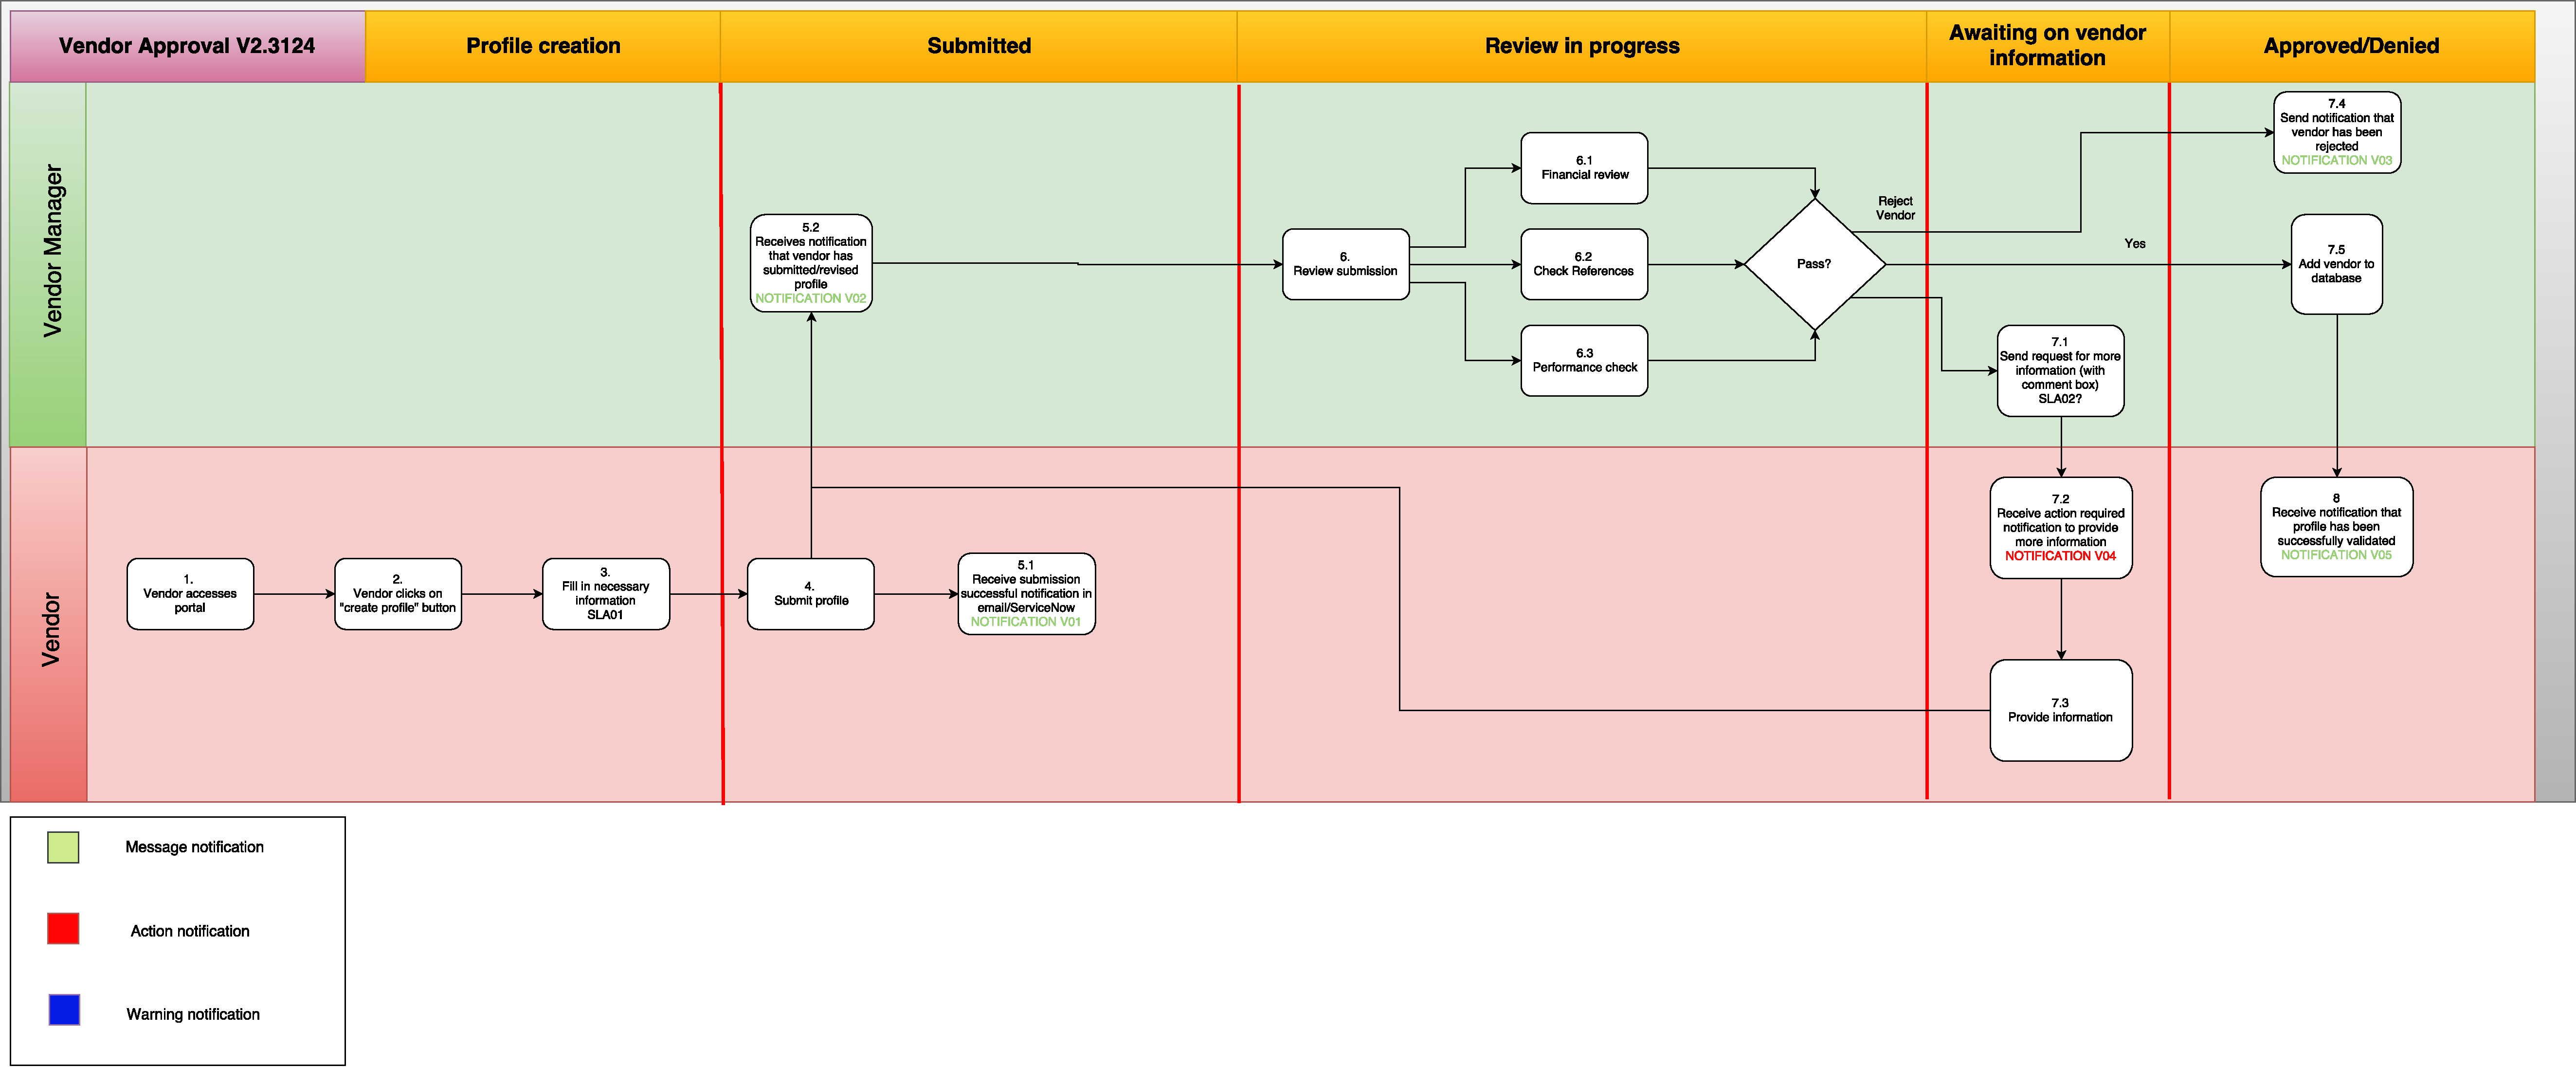
\includepdf[pages={-},angle=-90]{../Workflow/Vendor_Profile_Approval/Vendor_Profile_Approval_11_2.pdf}

\subsubsection{ Functional requirements}

\lipsum[10]

%----------------------------------------------------------------------------------------

%	System feature B

%----------------------------------------------------------------------------------------



\subsection{System feature B}

\subsubsection{Vendor Job Application}

After the vendor makes a profile now the vendor can apply to jobs from whats is available

\subsubsection{Action/result}

See Work-flow on the next page

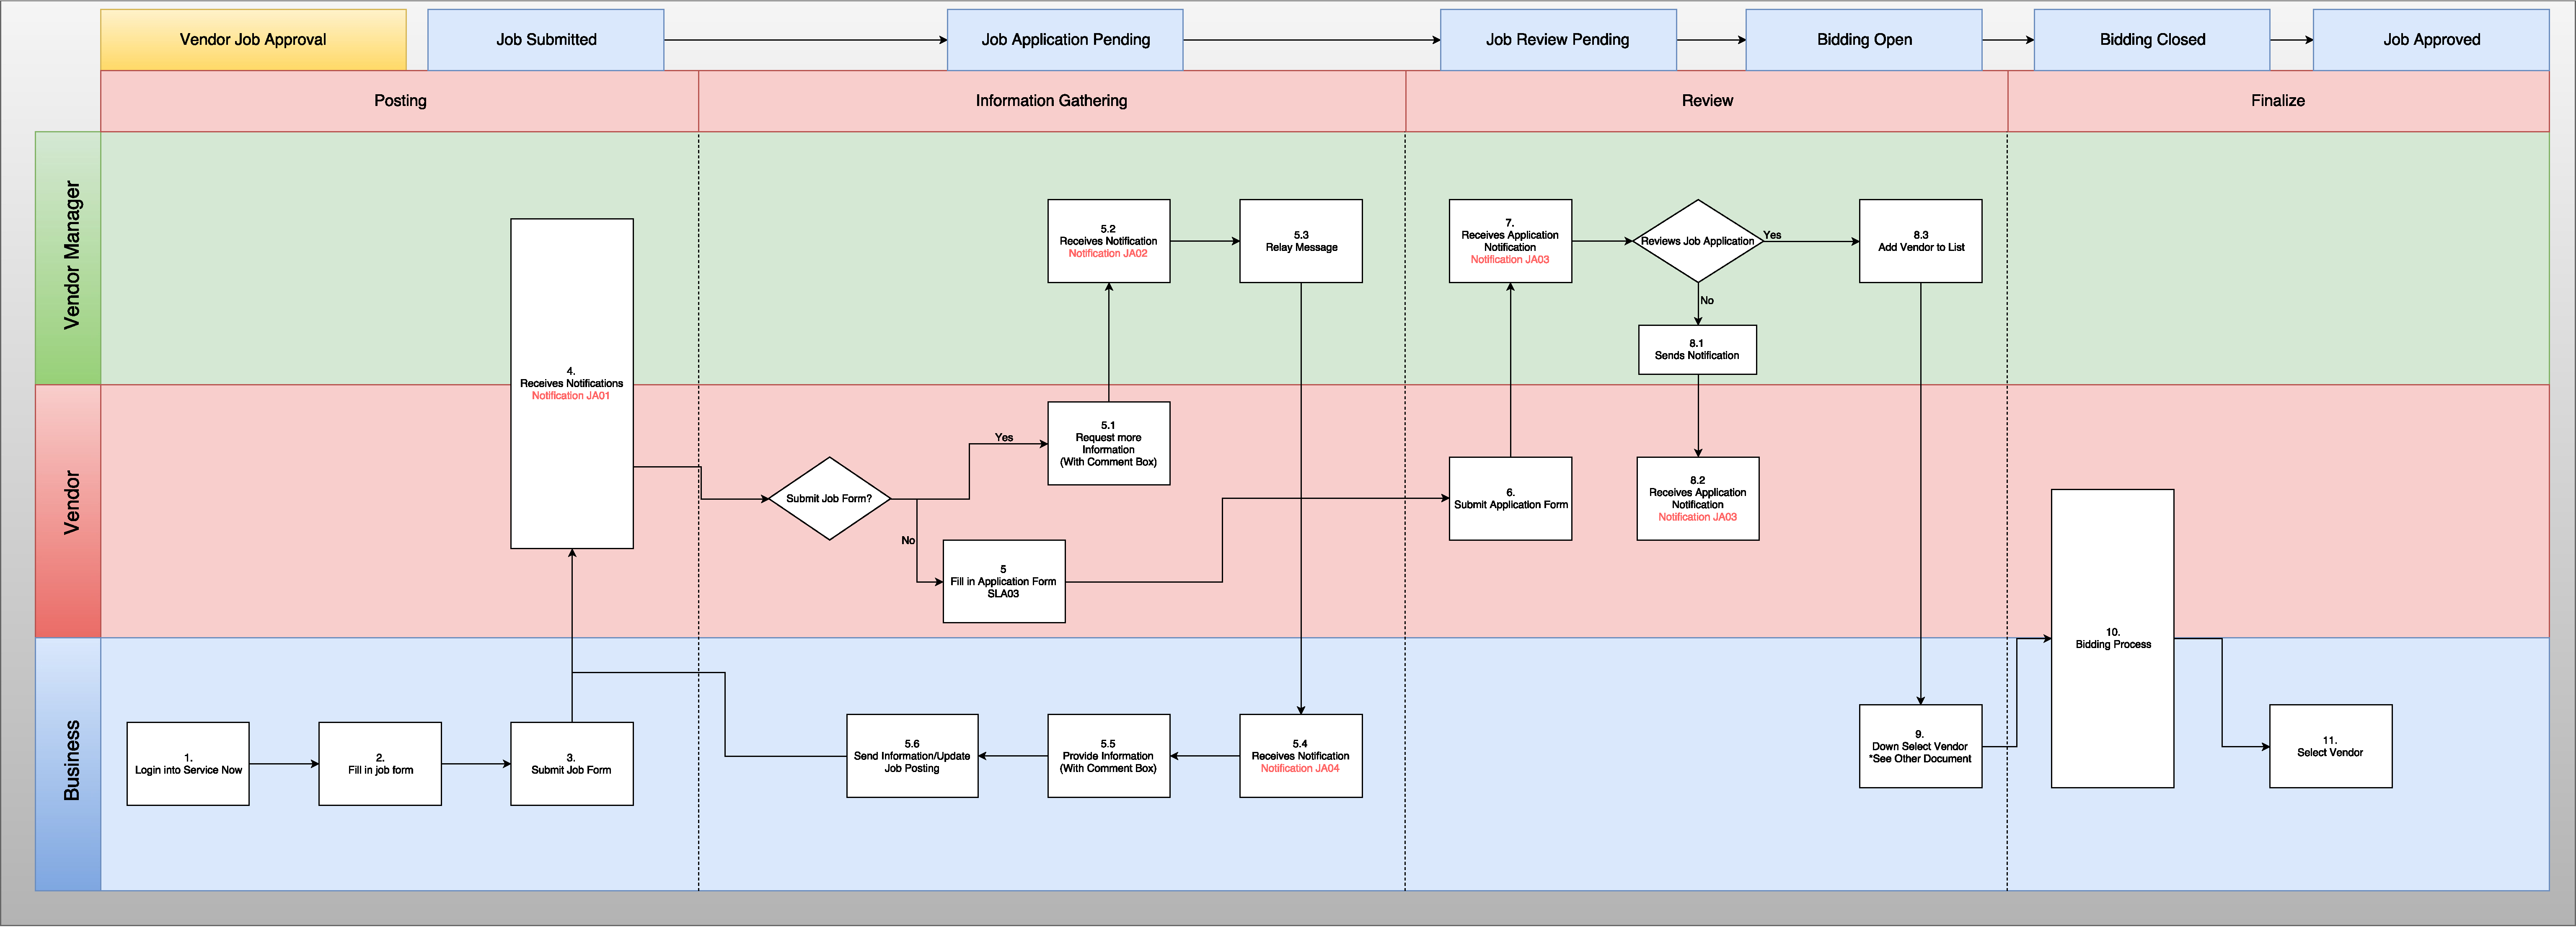
\includepdf[pages={-},angle=-90]{../Workflow/Vendor_Job_Application/Vendor_Job_Application_11_2.pdf}

\subsubsection{ Functional requirements}

\lipsum[10]



%----------------------------------------------------------------------------------------

%	Other

%----------------------------------------------------------------------------------------



\section{Other Nonfunctional Requirements}

\subsection{Performance requirements}

\lipsum[10]

\subsection{Safety requirements}

\lipsum[10]

\subsection{Security requirements}

\lipsum[10]

\subsection{Software quality attributes}

\lipsum[10]

\subsection{Project documentation}

\lipsum[10]

\subsection{User documentation}

\lipsum[10]

\section{Other Requirements}

\begin{appendices}

	\section{Performance requirements}

	\lipsum[10]

	\section{Safety requirements}

	\lipsum[10]

\end{appendices}



\end{document}
